%% Requires compilation with XeLaTeX or LuaLaTeX
\documentclass[10pt,xcolor={table,dvipsnames},t,aspectratio=169]{beamer}
\usetheme{NorthwesternKellogg}
\usepackage{IEEEtrantools}
\usepackage{mathtools}
\usepackage{caption}
\usepackage{graphicx}

%% Change Table %%
\usepackage{changepage}
\usepackage{array}
\usepackage{subfigure}

%% Get Hyperlink %%
\usepackage{hyperref}
\hypersetup{
    colorlinks=true,
    linkcolor=Purple,
    filecolor=Purple,      
    urlcolor=Purple
}

\newcolumntype{F}[1]{%
    >{\raggedright\arraybackslash\hspace{0pt}}p{#1}}%
\newcolumntype{T}[1]{%
    >{\centering\arraybackslash\hspace{0pt}}p{#1}}%

%% Insert Title Here %%
\title[Your Short Title]{Your Presentation}
\subtitle{Your subtitle (if there's one)}
\author{Your Name}
\institute{Your Faculty/Department}
\date{Date of Presentation}

\begin{document}

%% Document Setup %%
{
\setbeamertemplate{headline}{}
\setbeamertemplate{footline}{}
\begin{frame}[noframenumbering]
    \titlepage
\end{frame}
}


% Uncomment these lines for an automatically generated outline.
%\begin{frame}{Outline}
%  \tableofcontents
%\end{frame}

\section{Introduction}

\begin{frame}{Introduction}
\begin{itemize}
  \item Your introduction goes here!
  \item Use \texttt{itemize} to organize your main points.
\end{itemize}
\end{frame}


\section{Sections in \LaTeX}

\begin{frame}[c]{Insert Picture Here}
    \begin{figure}[H]
    \centering
    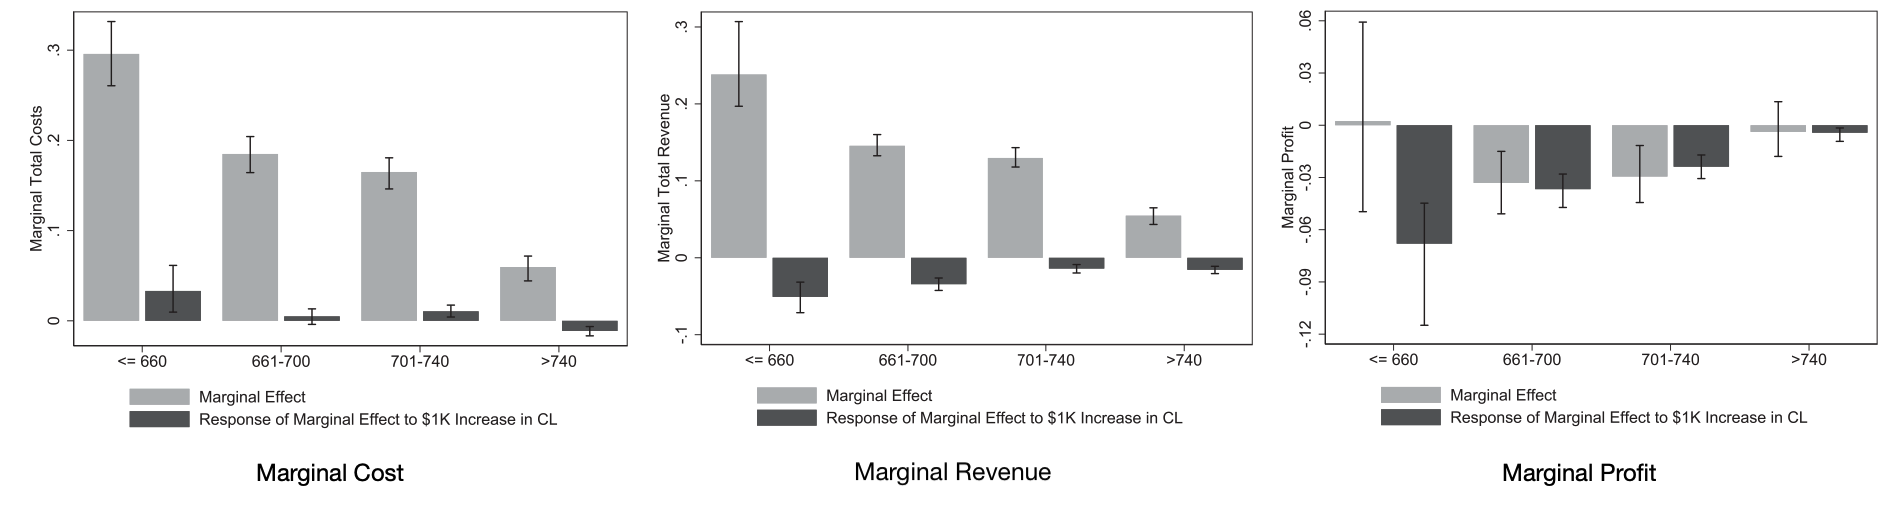
\includegraphics[width=1\textwidth]{fig/marginal_profit.png}
    \caption{Source: \href{https://academic.oup.com/qje/article/133/1/129/3950284}{Agarwal, et. al. (2018)}}
    \end{figure}
\end{frame}



\begin{frame}[c]{Insert Two Columns of Text/Figure Here}
\begin{columns}[T]
\column{0.49\textwidth}
\begin{itemize}
    \item Discontinuity in credit limit is not prima facie consistent with profit maximizing assumption!
    \item Makes more sense when considered in light of fixed cost of constructing scorecard for each subpopulation
    \item Discontinuities in credit limit is in line with industry practice (OCC, 2015)
\end{itemize}
\column{0.49\textwidth}
    \begin{figure}
    \centering
    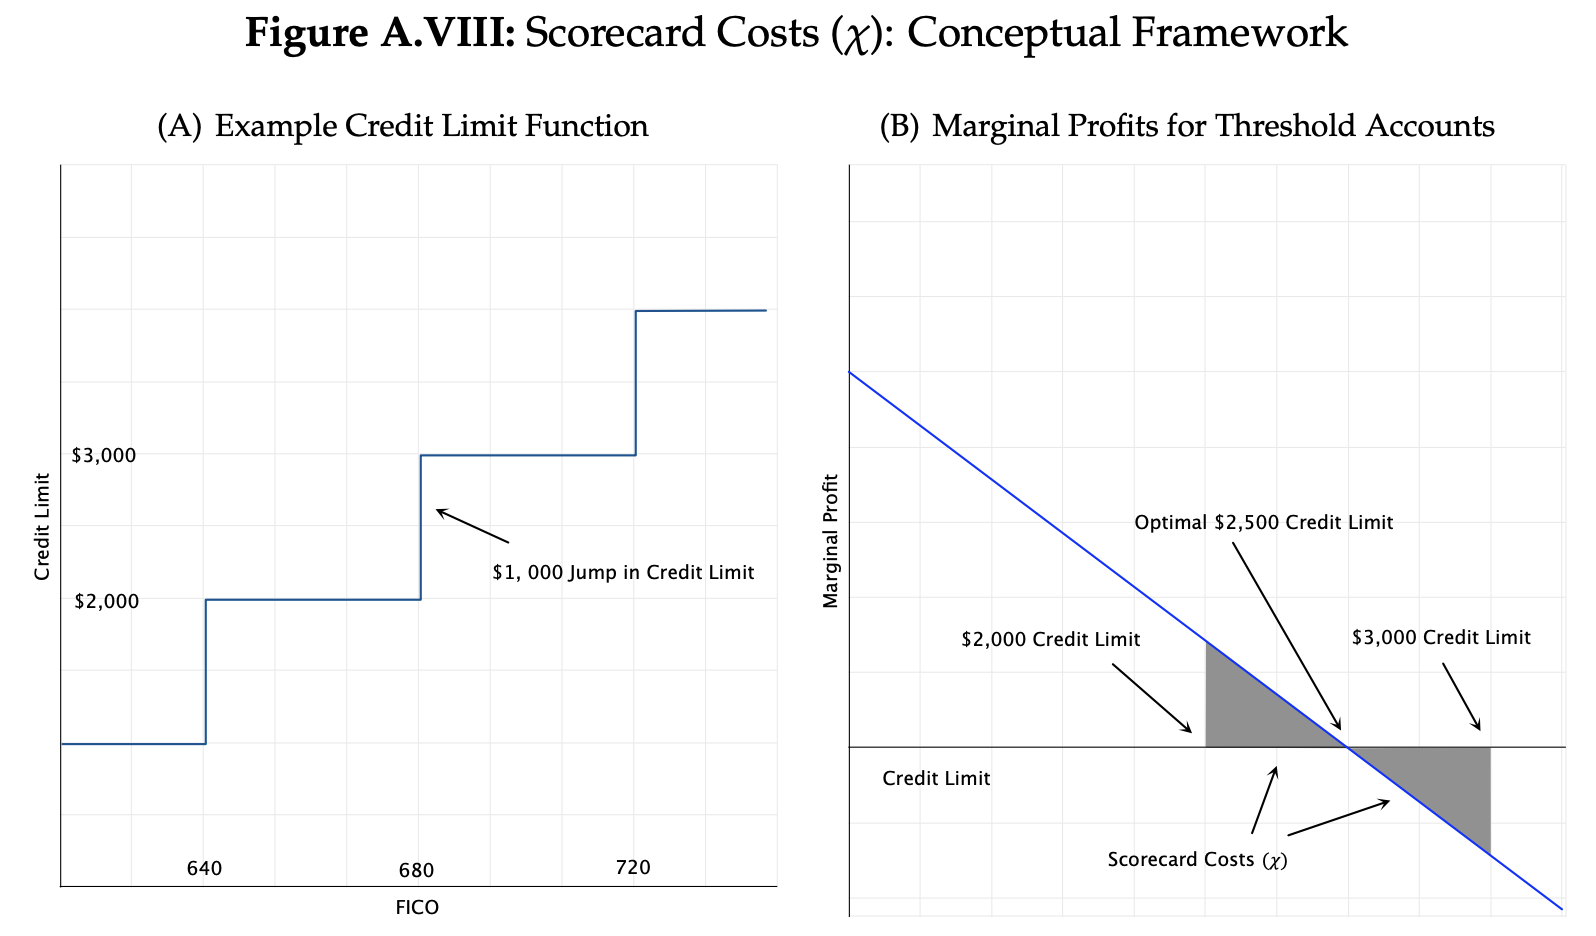
\includegraphics[width=\textwidth]{fig/scorecard_cost.png}
    \caption{Source: \href{https://academic.oup.com/qje/article/133/1/129/3950284}{Agarwal, et. al. (2018)}}
    \end{figure}
\end{columns}
\end{frame}


% Notes: remove [c] below if you want the table to be top-aligned vertically
\begin{frame}[c]{Insert Tables Here}
\begin{table}
\centering
\begin{tabular}{l r}
\tableheadrow
\tableheadcol{Item} & \tableheadcol{Quantity} \\
Widgets & 42 \\
Gadgets & 13
\end{tabular}
\caption{\label{tab:widgets}An example table.}
\end{table}
\end{frame}


\begin{frame}{Text in Two Columns}
\begin{columns}[T]

\begin{column}{0.49\textwidth}
Lorem ipsum dolor sit amet, consectetur adipiscing elit. Fusce sit amet massa in dolor pellentesque tempor. Integer nunc. 
\end{column}

\begin{column}{0.49\textwidth}
\begin{itemize}
\item First bullet goes here
  \begin{itemize}
  \item Secondary bullet goes here
    \begin{itemize}
    \item Tertiary bullet goes here
    \end{itemize}
  \end{itemize}
\end{itemize}
\end{column}

\end{columns}
\end{frame}

\begin{frame}[plain,noframenumbering,c]
\begin{center}
{\huge\rmfamily \textcolor{Purple}{Thank You!}}

\vspace{2em}
\textit{\small Contact: alvin.lumbanraja@kellogg.northwestern.edu}
\end{center}

\end{frame}

\end{document}
